\documentclass[letterpaper,twocolumn,10pt, anonymous]{article}
\usepackage{usenix2019_v3}

\usepackage{amsmath}
\usepackage{filecontents}
\usepackage{tikz}
\usepackage{xspace}
\usepackage{listings}
\usepackage{xcolor}
\usepackage{textcomp}
\usepackage{graphicx}
\usepackage{caption}
\usepackage{subcaption}
\usepackage{todonotes}
\usepackage{multirow}
\usepackage{booktabs}
\usepackage{paralist}
\usepackage{enumitem}
\usepackage{tabulary}
\usepackage{prettyref}
\usepackage{verbatim}
\usepackage{balance}
\usepackage{tabularx}

%-------------------------------------------------------------------------------
\begin{document}
%-------------------------------------------------------------------------------


\lstdefinestyle{cstyle}{
  basicstyle=\footnotesize\ttfamily,
  keywordstyle=\color{black!85}\bfseries,
  keywordstyle=[2]\color{black!85}\bfseries\emph,
  showstringspaces=false,
  language={C},
  breaklines=false,
  mathescape=true,
  escapechar={@}
}
\lstdefinestyle{inline}{
  style=cstyle,
  mathescape=false,
  breaklines=true,
  keywordstyle=,           
  keywordstyle=[2],
  extendedchars=true,
  basicstyle=\ttfamily\small
}
\newcommand{\Code}[1]{\lstinline[style=inline,breaklines=false]@#1@}
\let\realparagraph\paragraph
\let\paragraph\relax
\newcommand{\paragraph}[1]{\textbf{#1.}}
\newcolumntype{Q}{>{\centering\arraybackslash}X}
\newcolumntype{M}[1]{>{\centering\arraybackslash}m{#1}}

\newcommand\tocttou[0]{TOCTTOU\xspace}
\newcommand\tiktok[0]{TikTok\xspace}

\newrefformat{cha}{\hyperref[#1]{Chapter~\ref*{#1}}}
\newrefformat{sec}{\hyperref[#1]{Section~\ref*{#1}}}
\newrefformat{sub}{\hyperref[#1]{Section~\ref*{#1}}}
\newrefformat{tab}{\hyperref[#1]{Table~\ref*{#1}}}
\newrefformat{fig}{\hyperref[#1]{Figure~\ref*{#1}}}
\newrefformat{line}{\hyperref[#1]{line~\ref*{#1}}}
\newrefformat{lst}{\hyperref[#1]{Listing~\ref*{#1}}}
\newrefformat{pat}{\hyperref[#1]{Patch~\ref*{#1}}}
\newrefformat{alg}{\hyperref[#1]{Algorithm~\ref*{#1}}}

\renewcommand\itemautorefname{Attack}

\newcommand\mat[1]{\noindent{\color{blue} {\bf \fbox{Mat}} {\it#1}}}
\newcommand\atri[1]{\noindent{\color{red} {\bf \fbox{AB}} {\it#1}}}
\newcommand\UT[1]{\noindent{\color{violet} {\bf \fbox{UT}} {\it#1}}}

%don't want date printed
\date{}

% make title bold and 14 pt font (Latex default is non-bold, 16 pt)
\title{\Large \bf \tiktok: Systematic Kernel TOCTTOU Protection}

%for single author (just remove % characters)
\author{
{\rm Anonymous Submission \#94}
%Your Institution
% copy the following lines to add more authors
% \and
% {\rm Name}\\
%Name Institution
} % end author

\maketitle

%-------------------------------------------------------------------------------
\begin{abstract}
%-------------------------------------------------------------------------------
Double-fetch bugs are a plague across all major operating system kernels. They
occur when data is fetched twice across the user/kernel trust-boundary while 
allowing concurrent modification. Such bugs enable an attacker to illegally 
access memory, cause denial of service, or to escalate privileges. 
%
So far, the only protection against double-fetch bugs is to detect and fix them.
However, they remain incredibly hard to find. 
%
Similarly,
they fundamentally prohibit efficient, kernel-based stateful system call filtering.
% Mat: not a key argument for TikTok
% Even worse, the bug may be in
% unchangeable code (e.g., a binary driver blob).
%
We propose \tiktok to mitigate double-fetch bugs. \tiktok creates on-demand
snapshots and copies of accessed data, enforcing our key invariant
that throughout a syscall's lifetime, every read to a userspace object 
will return the same value.

\tiktok shows no noticeable drop in performance when evaluated on CPU-bound
workloads. On system call heavy workloads, \tiktok incurs 0.2-18\%
performance overhead, while protecting the kernel
against any \tocttou attacks. On average, \tiktok shows a $4.3\%$ overhead on
diverse workloads across two benchmark suites.

\end{abstract}

%%%%%%%%%%%%%%%%%%%%%%
\section{Introduction}
%%%%%%%%%%%%%%%%%%%%%%

The operating system (OS) kernel enables isolation between processes and is 
a key trusted computing
base. Each \emph{untrusted} userspace process runs under a
dedicated user in its own address space and must request resources such as
communication channels or changes to its address space from the \emph{trusted}
kernel. The userspace/kernel interface forms an explicit trust barrier
and all data that crosses this boundary in either direction must be carefully 
checked by the kernel.
%
Userspace processes attack the kernel by issuing system calls that then trigger
kernel bugs, elevating the privileges of the process.
%
A common class of kernel bugs are so-called \emph{double-fetch}
bugs~\cite{serna08doublefetch, twizsgrakky07ring0, wilhelm2016xenpwn,
wang2018survey}. They occur when higher-privileged code, such as
the kernel, reads the same data from the lower-privileged address space twice.
%
Double-fetch bugs are a type of
\emph{race condition} between threads of different privileges. A
\emph{Time-of-check to time-of-use (\tocttou)} violation occurs when the first
read is used to check a condition while the second read is used to modify
state.
%
An example of a double fetch bug is when the kernel reads the length of a buffer
from userspace, allocates a kernel buffer, then reads the length a second time
to finally copy the data from userspace to kernel. An adversary may concurrently
overwrite the length of the buffer to a larger number after the kernel allocated
its buffer, causing the memory copy to overflow the buffer.
%
Double-fetch bugs are a frequent problem in kernels and
hypervisors~\cite{cve201812633, cve202012652, cve20131332, cve201920610,
cve20158550, cve201610439, cve201610435, cve201610433, cve20195519,
cve20168438}. 
% Considering that double-fetches also appear in drivers, legacy
% systems with binary-only drivers cannot be patched, even if a bug is found.
Watson~\cite{watson2007exploiting} blames an unfixable \tocttou
constellation as a reason for the generic insecurity of \emph{system call
wrappers}. 
System call filtering wrappers require that data read from userspace for the
initial check remains the same when the kernel later uses it for computation, 
and can currently only check arguments passed by value.
\tiktok enables ``deep argument inspection'' for SecComp~\cite{seccomp_deep, seccomp}
i.e., checks on arguments passed by reference.
Without \tiktok, such inspection is inherently impossible since such checks 
introduce double fetches, and consequently \tocttou bugs.

To mitigate double-fetch bugs in the kernel, a system must prohibit
\emph{concurrent changes} to memory accessed by the system call. Adversaries may
find thrifty ways to trigger such concurrent writes:
\begin{inparaenum}[\itshape i\upshape)]
\item  direct writes from userspace (e.g., from concurrent threads),
\item  kernel writes from system calls (e.g., from concurrent system calls),
\item  modifying address space mappings,
\item  concurrent \texttt{write}s to a file that alters mapped
file pages, or
\item  storing arguments on device-backed pages, leveraging devices to trigger
concurrent writes.
\end{inparaenum}
To prevent attacks, all kinds of concurrent writes must be prohibited.

% TODO key idea
We base our defense on a single key invariant: 
\textbf{\emph{through a syscall's lifetime, every read to a userspace object 
will return the same value}}. Based on this invariant we derive a \emph{security
property} that ensures that every read during the execution of a system call is
tracked. Subsequent reads of the same address will always return the same value.
For performance, multiple versions of an object may exist at the same time
depending on when the system call was started and depending on how many
concurrent system calls are in flight. Orthogonal, we derive a \emph{correctness
property} that ensures the sharing of the correct version among the different
system calls that are in flight. All writes end up on the most recent version of
the objects and therefore allow forward progress.
% Mat: should we split it into security, correctness, and performance
% properties, all driven by the core invariant?
We implement our invariant in our \tiktok prototype for the Linux kernel, but
the defense applies to any modern operating system kernel.

Our evaluation shows overall low performance overhead for our mitigation.
On parallel workloads from the NAS Parallel Benchmarks suite, \tiktok shows 
an average performance overhead of $3.7\%$ while its performance overhead on
more kernel-intensive workloads from the Phoronix Test Suite is $5\%$ with 
negligible memory overhead.
The security evaluation demonstrates how \tiktok successfully stops all attacks
against vulnerable system calls, along with providing the developer with
sufficient information about the location of the bug.
%
The main contributions of this paper are:

\begin{itemize}[noitemsep]
\item Distillation of \tocttou attack vectors into a core invariant that protects
the kernel against malicious concurrent modifications;
\item \tiktok, a design that prohibits and detects
\tocttou attacks against modern kernels, prohibiting their exploitation,
enabling developers to detect \tocttou bugs, and providing the foundation for
safe system call interposition and validation;
\item An efficient implementation of \tiktok for the Linux kernel that exhibits
low ($3.7\%$) performance overhead.
\end{itemize}


%%%%%%%%%%%%%%%%%%%%
\section{Background}
%%%%%%%%%%%%%%%%%%%%

\tiktok orchestrates several mechanisms within the Linux memory subsystem 
to provide its protection guarantees.
Linux uses architecturally defined per-address space page tables to define
mappings to pages.
\tiktok protects these pages by temporarily marking them read-only in the 
page tables.
This section provides the background information necessary to reason about 
why and how \tiktok protects syscalls from concurrent writes.


\subsection{Page Tables and Memory Protection}
%%%%%%%%%%%%%%%%%%%%%%%%%%%%%%%%%%%%%%%%%%%%%%

Virtually all modern architectures (e.g., x86, ARM, SPARC, and 
RISC-V) implement separate virtual and physical
address spaces (AS) based on fixed-size regions called pages.
%
Some architectures also include segmentation-based protection 
working in tandem with page tables, but segmentation is irrelevant for \tiktok.
%
Programs execute in their virtual address space while caches and main memory
are accessed using physical addresses.
Architectures rely on page tables orchestrated by the operating system 
to translate between these address spaces and to protect such accesses.
Page tables are arranged as radix trees where different bits of the 
virtual address are used as indices into levels of the page table.
At the leaf page table, a unique pagetable entry (PTE) stores the 
translation and protection information for a page.

A PTE in x86-64 is a 64-bit value holding, among others, the following metadata:
% \begin{description}[noitemsep]
%   \item[Present bit (P)] which marks the PTE's validity;
%   \item[Protection bits (NX, R/W, U/S)] which restrict the type of
%         access and the privilege level of the accessing code;
%   \item[Software-usable bits] (SW1-SW4) ignored by the MMU and used by the 
%         operating system to store metadata;
%   \item[Page Frame Number (PFN)] identifying the page's physical address.
% \end{description}
a \emph{Present bit (P)} to mark the PTE's validity;
\emph{Protection bits (NX, R/W, U/S)} to restrict the type of
access and the privilege level of the accessing code;
\emph{Software-usable bits (SW1-SW4)} that are ignored by the MMU and used by the 
operating system to store metadata; and
\emph{Page Frame Number (PFN)} to identify the page's physical address.

An access using a virtual address first reads the corresponding PTE's 
present bit to check its validity. 
Then, the access checks whether the access is allowed from the executing
code's privilege level by checking the U/S bit and whether the 
read/write access is allowed by checking the R/W bit.
When all checks pass, the processor uses the PFN to find the data in 
the caches or in memory.
When a check fails, the processor raises a protection fault/exception and
moves control to a OS-specified exception handler.

Reading PTEs from a multi-level page table is an expensive operation, and 
modern processors cache PTEs in caches known as Translation Lookaside 
Buffers (TLBs) to reduce the cost of subsequent accesses. 
On most architectures, the OS is responsible for keeping TLBs coherent with 
the page table, necessitating entries to be flushed from TLBs when the 
corresponding PTE is updated.


\subsection{Linux Memory Subsystem}
%%%%%%%%%%%%%%%%%%%%%%%%%%%%%%%%%%%

Linux implements various abstractions, such as processes, files, and shared
memory using the architecture's page tables.
All threads within a Linux process share a single address space, and 
consequently use the same page table for translation and protection.
Each page within the process' virtual address space may be mapped or 
unmapped, and mapped pages have separate read/write/execute permissions.
Generally, programs have write-execute exclusion which means that 
code pages cannot be written to and data pages cannot be executed.
These permissions map directly to page-table bits.
Pages in Linux may also be copy-on-write pages which are mapped read-only
in multiple address spaces, but duplicated when any process writes
to it, resulting in a separate copy.

Linux maintains userspace and kernel mappings to memory in distinct 
parts of the virtual address space. 
The top half of the address space holds kernel mappings, and the 
PTE entries for such pages have the U/S bit set. 
The kernel mappings are identical for all address spaces, and are 
kept consistent across the corresponding page tables.
The bottom half of the address space is used for userspace mappings, 
and the PTE entries have the U/S bit reset.
A userspace page has at-least one userspace mapping, and at-least one
kernel mapping.
Shared userspace memory is implemented by mapping a page in more than 
one address space.

Files in Linux occupy a separate namespace as that of virtual memory
(rooted at \Code{/}).
However, when files are read or written, parts of the file are cached
in the kernel's page cache consisting of pages mapped in the kernel's 
address space.
Further, programs can explicitly map pages from a file, in which case 
the corresponding pages from the page cache are also mapped in userspace 
addresses in the process' page table.
Mapped file pages can therefore be accessed by the file-system driver using 
kernel addresses, and userspace programs using userspace addresses.
Userspace pages not backed by a file are called anonymous pages.


\subsection{Supervisor Memory Protection} %  and user-copy interfaces}
%%%%%%%%%%%%%%%%%%%%%%%%%%%%%%%%%%%%%%%%%%%%%%%%%%%%%%%%%%%%%%%%%%%

Kernel accesses to userspace memory use userspace mappings, and 
come with the risk of the kernel confusing data structures 
stored in userspace memory for actual kernel data structures.
A class of attacks can exploit this behavior via bugs in the 
kernel.
Essentially, the adversary needs to set up either data structures
or code within its accessible memory, then exploit a kernel 
bug to make the kernel use these data structures, or to execute 
this code.

Architectures and OSs have mitigated this class of vulnerabilities
by introducing Supervisor Memory Protection.
Essentially, kernel read/write/execute access to userspace memory
raises a fault depending on the state of a per-core system 
register.
On x86-64, these features are known as Supervisor Memory Access 
Protection (SMAP) for data accesses and Supervisor Memory Execution 
Protection (SMEP) for code accesses, and bits in the CR4 register 
are used to enable/disable the features.
The architecture also exposes privileged instructions 
\Code{stac}/\Code{clac} to quickly disable and enable this access 
control.
On the OS side, all accesses to userspace memory are made explicit, 
using special functions to read from and write to userspace memory.
Any unintended access, outside these functions, causes a 
hardware fault, indicating either a kernel bug or an attack.
Linux implements the functions \Code{copy_\{from/to\}_user} which 
use the access control instructions to disable SMAP before 
accessing userspace data, and then re-enabling SMAP afterwards.
Kernel accesses to userspace data therefore become explicit, allowing
\tiktok to reliably track all kernel fetches from userspace memory, 
and therefore protect them.


\subsection{Double-Fetch Bugs}
%%%%%%%%%%%%%%%%%%%%%%%%%%%%%%

\begin{figure}[]
  \centering
  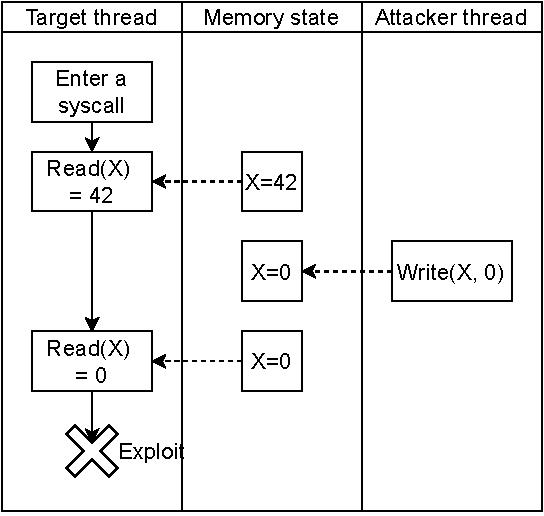
\includegraphics[width=.8\linewidth]{img/doublefetch.pdf}
  \caption{Example of a double-fetch bug.}
  \label{fig:doublefetch}
\end{figure}

Double-fetch bugs occur when a privileged environment (such as the kernel)
reads untrusted memory two or more times, and the read values are not 
identical. 
An example of such a situation is depicted in \autoref{fig:doublefetch}.
In between two reads by the target thread, the value of \Code{X} in memory 
is changed by an adversary.
The bug is a race condition since it requires accesses to memory in 
a particular order across threads.
The situation where the first fetch validates an object's value in memory and 
the second fetch uses the same object's value is called a 
\emph{Time-of-check to time-of-use (\tocttou)} bug.
\tocttou bugs have been widely studied in file systems, where the 
API makes it possible to swap the file after validating the access 
rights~\cite{payer2012protecting,
pu2006methodical, wei2010modeling, tsafrir2008portably}.
\tocttou bugs affect kernel code~\cite{jurczyk2013bochspwn, wang2018survey}
as well as dynamically loaded driver code~\cite{cve201812633,cve201812633fix}.
Wang et al.~\cite{wang2018survey} showed that double-fetches appear not only
in kernels, but wherever there is a trust boundary to cross (e.g., kernel ---
hypervisor~\cite{wilhelm2016xenpwn} and hardware---kernel
boundaries~\cite{lu2018untrusted}). 


%%%%%%%%%%%%%%%%%%%%%%%%%%%
%\section{Attack vectors}
%\label{sec:threats}
%%%%%%%%%%%%%%%%%%%%%%%%%%%

% In this section, we describe the threat model for exploiting double-fetch
% bugs in the kernel and classify the possible attacks based on how the 
% data is modified between vulnerable double-fetches.

\section{Threat Model}
\label{sec:threatmodel}
%%%%%%%%%%%%%%%%%%%%%%%%%

% Nothing fancy -- the adversary is just trying to hack the system
% No black magic allowed
The adversary has access to a user account on the target machine. They can
execute arbitrary userspace code, including system calls. Some of the system 
calls have double-fetch vulnerabilities, and the adversary wants to exploit them,
e.g., for privilege escalation.
The adversary may execute arbitrary sequences of system calls on multiple CPU
cores concurrently.

\tiktok mitigates any unintended corruption or information leakage \emph{in the kernel}
or \emph{in other user processes} that arises through double-fetch bugs. 
Hardware attacks such as Rowhammer~\cite{mutlu2019rowhammer}
or side-channels~\cite{kocher2019spectre}, and file-system TOCTTOU
attacks~\cite{payer2012protecting, pu2006methodical, wei2010modeling,
tsafrir2008portably} are out of scope.


\section{Attack Classification}
\label{sec:attacks}
%%%%%%%%%%%%%%%%%%%%%%%%%%%%%%%%%%

\begin{table}
  \begin{center}
    \begin{tabular}{  l  M{12mm}  M{20mm}  M{20mm} }
  \toprule
      & \textbf{Userspace} & \textbf{Kernel} & \textbf{Device} \\ \cmidrule{1-2} \cmidrule{3-3} \cmidrule{4-4}

      % Note: this is a manually tuned fixup. multirow just sucks.
      \multirow{2}{*}[-.8em]{\shortstack{\textbf{Existing} \\\textbf{mapping}}} 
      & Intra AS      & User mapping   & Device page       \\ \cmidrule{2-4}
      & Cross AS      & Kernel mapping & Device DMA page   \\ \cmidrule{1-4}
      \multirow{2}{*}[-2.4em]{\shortstack{\textbf{New} \\\textbf{mapping}}} 
      & mmap          & mm\_populate   & New device page   \\ \cmidrule{2-4}
      & clone         & --             & New device DMA    \\ \cmidrule{2-4}
      & swap          & --             & New device DMA    \\ 
  \bottomrule
  \end{tabular}
  \end{center}
  \caption{Attack vector classification for \tocttou exploits.}
  \label{tab:attack_class}
\end{table}

\tiktok guards data processed during a syscall's execution against concurrent modification.
We denote the data fetched twice as vulnerable data.
In this section, we classify attacks based on two criteria: the 
privilege level of the writer, and whether the mapping used for writing 
existed at the time of the first read (see \autoref{tab:attack_class}).
This classification helps understand existing attacks and how to 
protect against them, and where future attacks (bugs) may arise.
The device column corresponds to attacks where a device 
(e.g., a network card, GPU, or FPGA) is responsible for modifying vulnerable data.

Existing userspace mappings to a page can be used to modify 
vulnerable data which the targeted syscall is reading.
Userspace can directly write to a mapped page, whether that mapping is 
in the same or in a different address space. 
Such attacks are called \emph{direct double fetch} 
attacks~\cite{watson2007exploiting}.
Alternatively, a concurrently executing syscall can also modify the 
vulnerable data in a confused-deputy attack.
When the adversary passes a pointer to the vulnerable data to 
the syscall as a user-buffer in which the syscall can return some 
data, the kernel's write to the buffer can modify vulnerable data.
For example, the \Code{read} system call takes an argument pointing 
to a user buffer where the contents of a file will be copied to.
Another example is \Code{rt_sigaction} where the kernel writes to 
a user buffer pointed to by the \Code{oldact} argument.
In both of these attacks, the adversarial write uses a userspace
mapping. 
\emph{A protection mechanism must, therefore, account for all userspace 
mappings to pages containing vulnerable data at the time of the 
targeted syscall's first read.}

Existing kernel mappings to a page also mapped in userspace can be 
leveraged by an attacker in a confused-deputy attack.
The adversary maps a file-backed page from the page-cache in a
userspace process and then passed as an argument in this page to the 
targeted syscall.
The adversary then triggers a concurrent \Code{write} syscall to modify the 
vulnerable data using kernel mappings for the page-cache
pages~\cite{watson2007exploiting}.
% This attack is called \emph{inception double fetch}~\cite{watson2007exploiting}.
% \mat{Did we call it inception double fetch?}
The kernel does not explicitly track kernel addresses mapping to a page, 
but the file-system driver does explicitly find the page before writing to it.
\emph{A protection mechanism must, therefore, instrument file-system 
drivers to account for writes via kernel mappings to vulnerable data.}

The kernel might create new mappings to the vulnerable data 
between the double fetches by the target syscall, bypassing protection 
mechanisms which instrument the first read to protect the accessed page.
An adversary can call \Code{mmap} and \Code{clone} syscalls to create 
a new mapping to the vulnerable data before writing to it.
The first version is called a \emph{reflected double fetch} 
attack~\cite{watson2007exploiting}.
The mapping might not be created at the time of the adversarial syscall, 
but lazily when the attacker writes to the vulnerable data.
In a more involved variant, the adversary can use the kernel as a 
confused deputy which touches the unmapped page and maps it in, 
then writes to the vulnerable data.
In all of the above vectors, the function populating pages for a 
process (\Code{mm_populate} for Linux) is creating the new mapping.
\emph{A protection mechanism must, therefore, instrument \Code{mm_populate}
and the code of any other syscall which may create new mappings.}

A new mapping might also be created due to swapping.
If the adversary writes to a page that was previously swapped 
to disk, but later swapped in to be read by the target syscall in 
a different address space, the kernel might lazily reinstate 
the adversary's mapping to the page.
\emph{The swapping mechanism must, therefore, be protected.}

\tiktok protects against all of the aforementioned attack vectors.
In the absence of any other syscall which can create new userspace 
mappings to vulnerable data, \tiktok's protection is complete 
against writes from both user and kernel code.

Finally, a device might modify vulnerable data if it is either 
allowed to DMA to the page, or if the page is memory-mapped and is 
actually backed by the device.
In the latter case, external factors can change the vulnerable 
data.
Existing discretionary access control rules generally bar users 
except a superuser from mapping device-backed pages into their
address spaces.
Such users are also disallowed from configuring DMA devices.
Therefore, device modifications to vulnerable data fall outside 
our threat model and are not protected by \tiktok.
As a superuser can modify kernel code, protecting against attacks from the
superuser is outside of our threat model.
% The superuser may load arbitrary kernel code % via loadable
% % modules
% and confused-deputy attacks leveraging an incompetent 
% system administrator are also outside the purview of our threat model.
However, on processors supporting IOMMUs, \tiktok can be extended 
to protect against modifications by DMA devices.


%%%%%%%%%%%%%%%%%%%%%%%%%%%
\section{\tiktok Design} 
\label{sec:design}
%%%%%%%%%%%%%%%%%%%%%%%%%%%

\tiktok maintains a single core \emph{invariant}:
\textbf{\emph{Through a syscall's lifetime, every read to a userspace object 
will return the same value}}.
By construction, the invariant guarantees that double-fetches in syscall
code will read the same data, \emph{eliminating \tocttou bugs}.
\tiktok maintains the invariant by tracking \emph{snapshots} of objects
when first accessed, lazily making \emph{copies} when the object is concurrently 
written and accessing the correct copy on subsequent reads.
Copies are only maintained during syscalls' lifetimes, and are released as 
soon as no syscall needs it.
Consequently, each userspace object has a single copy when no syscalls are
running.
The invariant also means that only accesses to userspace objects by the kernel
need to be protected. 
Accesses to userspace objects from userspace and kernel objects by kernel 
code remains unaffected.

\tiktok's implementation builds on the protection mechanisms provided by 
existing virtual memory implementations.
On modern platforms, virtual memory protection is set up by the OS at
page-granularity by setting bits in pagetable entries (PTEs).
These permission bits are checked by the hardware on memory access, 
efficiently enforcing the permissions, and raising a fault when they 
are violated.
For efficiency, \tiktok implements its invariant at page-granularity, not object 
granularity: when a syscall reads from userspace, every page touched by that 
read is covered, not merely the bytes read.
As a side-effect of its implementation, \tiktok does not distinguish
accesses to different parts of a page, and may incur performance overhead due
to false sharing within a page. 
Page-granularity protections are more conservative compared to byte-granularity
protection and, therefore, \tiktok maintains its invariant nonetheless but may
incur performance overhead for false sharing on highly contended pages.

For an object spanning multiple pages, \tiktok's design sequentially 
protects each page before reading from it.
The leading pages containing the object are protected before the
later pages, allowing an adversary to potentially modify the later 
pages before the syscall first reads them.
However, the adversary is prevented from modifying any of these pages
after the syscall's first read, ensuring that double-fetches respect
the invariant.
If the syscall code contains a \tocttou bug, the modification will
be visible to the first fetch itself (which is used for checking for 
validity of the data) and will lead to the data being rejected 
straightaway.
\tiktok's invariant therefore prevent exploitation of double-fetch
vulnerabilities even when the fetched objects span multiple pages.

A major requirement for \tiktok is to allow concurrent access to pages
by user/kernel code running in parallel with a syscall which reads from 
the same pages.
This requirement prevents deadlocks and improves performance vis-a-vis
a na\"ive design which blocks all other tasks writing to pages already 
read by a syscall until the syscall completes.
The na\"ive design can deadlock because it introduces dependencies between
tasks for forward progress, which we illustrate in the following example
of a system with two tasks (A and B):
\begin{inparaenum}[\itshape i\upshape)]
  \item Task A issues a blocking system call which reads a user page and blocks, then
  \item Task B writes to the same user page before issuing a syscall which 
  resumes task A. 
\end{inparaenum}
In this case, if Task A's read to the page preceeds Task B's write, 
Task B will be blocked waiting for A to complete its syscall.
Task A will also remain blocked waiting for Task B's syscall, 
introducing a circular dependency, leading to deadlock.
The na\"ive design also introduces unnecessary delays in other cases, 
such as the one described below, again with two tasks (C and D):
\begin{inparaenum}[\itshape i\upshape)]
  \item Task C reads from a page and sleeps for a long while,
        but does not read from the page a second time, then
  \item Task D writes to the same page after task C has read from it, 
        and blocks until Task C completes and is unnecessarily delayed.
\end{inparaenum}
A more performant approach is to duplicate the concurrently accessed page: 
the copy is kept for task C for future fetches, and task D
can write to the original and proceed without delays.

\tiktok must maintain multiple versions of a page read by a syscall 
to maintain its invariant in the face of concurrent writes.
\tiktok introduces \emph{snapshots} and \emph{copies} to keep track 
of page versions. 
Snapshots are logical views of the page's contents at a particular time,
while the actual contents are stored in one of many copies. 
Each snapshot maps to a copy, allowing the contents of the page at the 
time of creating the snapshot to be read. 
If multiple snapshots are taken without intervening writes to the page, 
these snapshots will map to a single copy, reducing \tiktok's space overheads 
and performance overheads for creating copies.
\tiktok maintains a snapshot of every page when first read by a syscall.
On a double fetch by the same syscall, the copy mapped to the snapshot 
is accessed, ensuring that the data read is the same as the first time.
The latest copy of the page is used for all writes, by the syscall as 
well as from concurrently running tasks, updating the page as seen 
from userspace.
%
\tiktok's design draws parallels to multi-version concurrency control 
methods for databases based on snapshot isolation~\cite{0001MK15}.
Transactions read from a snapshot of the database state from when 
they started, and writes update the up-to-date state of the database.
%
\emph{Essentially, \tiktok is a multi-versioning system for pages where 
syscalls read from immutable versions to prevent \tocttou bugs and
syscalls and userspace both write to a single mutable version 
holding the latest state of the page.}

\subsection{Page State Machine}

\begin{figure*}[]
  \centering
  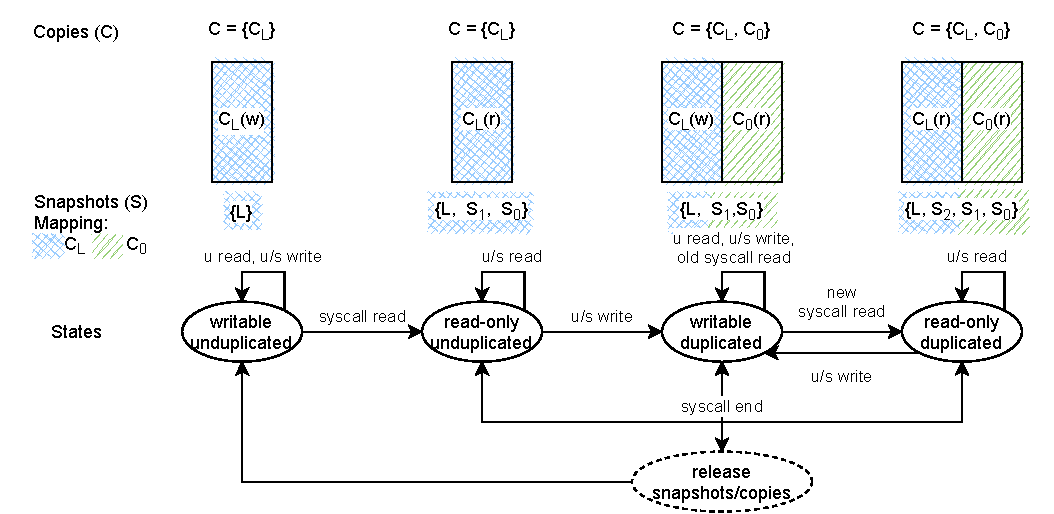
\includegraphics[width=0.9\linewidth]{img/tiktok_states.pdf}
  \caption{State diagram for a page in \tiktok. Reads/writes from userspace/syscall 
          code are marked (u)/(s) respectively. Shading is used to represent the 
          mapping from snapshots to copies.}
  \label{fig:tiktok_states}
\end{figure*}

\begin{figure}[h]
  \centering
  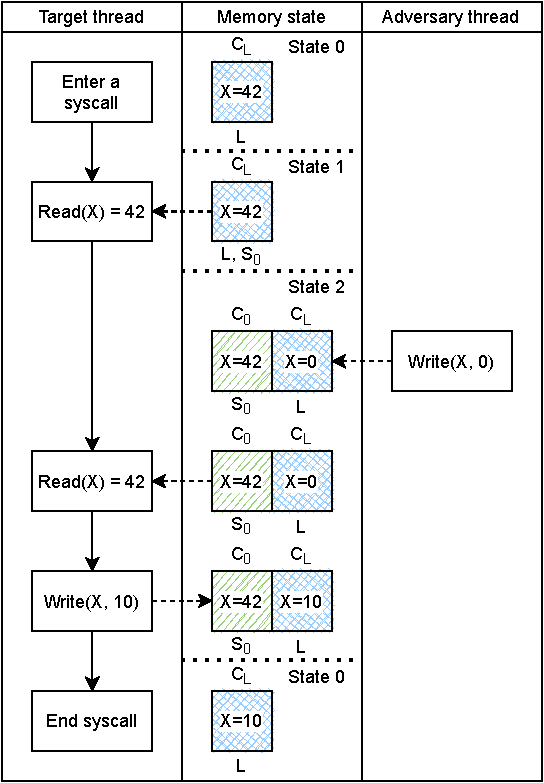
\includegraphics[width=\linewidth]{img/doublefetch_tiktok.pdf}
  \caption{Diagram illustrating \tiktok preventing exploitation of a double fetch.}
  \label{fig:doublefetch_tiktok}
\end{figure}

To track multiple versions of the contents of a page when being concurrently 
accessed by numerous tasks, from userspace or during a syscall,
\tiktok implicitly maintains a per-user-page state machine.
For a page, its corresponding state machine 
\begin{inparaenum}[\itshape i\upshape)]
  \item tracks snapshots for currently executing syscalls which have read it, 
  \item tracks copies of the page, and 
  \item maintains the mapping between snapshots and copies necessary for providing 
  the correct contents to subsequent reads. % by these syscalls.
\end{inparaenum}

\autoref{fig:tiktok_states} shows the state machine for a single page.
At every state, the page has two associated sets:
\begin{inparaenum}[\itshape i\upshape)]
  \item the copies set $C = \{C_L, C_0, \dots\}$ holds multiple copies of the page over time, and
  \item the snapshots set $S = \{L, S_0, S_1, \dots\}$ tracks logical versions of the page, each corresponding to one executing syscall and mapping to a copy. 
\end{inparaenum}
Reads from kernel code in a syscall use the \emph{snapshot's corresponding copy}.
Writes from user/kernel code and reads from userspace access the \emph{latest 
copy} $C_L$, which is mapped in processes' address spaces.
All other copies are read-only (no matter what the original page protection is), and are used for providing snapshots to syscalls.
Read-only pages only use states 0 and 1, and writes lead to segmentation faults
as they do on non-\tiktok systems.
Knowing which state the page is in allows \tiktok to differentiate faults due
to protecting pages from faults due to programs actually writing to an 
originally read-only page.
The latest copy $C_L$ of read-only pages remains read-only in both
protected states (1 and 3).
In the following paragraphs, we describe how the state machine for a single, 
writable user page transitions between its states, what triggers each transition, 
and what changes are made to the copies and snapshot sets on a transition.
In \autoref{fig:doublefetch_tiktok}, we illustrate how the state machine protects the 
syscall from \autoref{fig:doublefetch}.

\paragraph{State 0}
A page starts as \texttt{(unprotected, unduplicated)}.
In this state, there is a single copy $C_L$ and a single ``snapshot'' $L$. 
The snapshot $L$ refers to the latest version of the page which changes 
over time, and is the only mutable snapshot.
All processes where this page is mapped have unrestricted userspace read and write 
access, and unrestricted kernel write access.
The remaining operation, a read from kernel code, triggers a transition to 
State 1.
In \autoref{fig:doublefetch_tiktok}, the snapshot $L$ initially contains 
the value $42$.

\paragraph{State 1}
The page in State 0 transitions to the \texttt{(protected, unduplicated)} state as soon as a syscall 
reads from it.
\tiktok first marks the page's latest copy $C_L$ read-only in all processes, 
trapping writes to the page but allowing concurrent userspace reads to continue.
A new snapshot, $S_0$ linked to this syscall is allocated for this page.
For the rest of its lifetime, this syscall will only read from this snapshot.
Both snapshots $S_0$ and $L$ refer to the same copy $C_L$ (shown by the 
blue cross-thatch in \autoref{fig:tiktok_states}).
Prior to any writes to this page, any other syscalls which also read the page  
get their own snapshots (e.g., $S_1$) all pointing to the single copy $C_L$.
The page's read-only status causes the hardware to fault on any write,
notifying \tiktok to transition the page to State 2.
In \autoref{fig:doublefetch_tiktok}, the page transitions to State 1 when 
the syscall first reads it, and adds a snapshot $S_0$.

\paragraph{State 2}
A page in State 1 transitions to the \texttt{(unprotected, duplicated)} state 
on any write from user or kernel code.
\tiktok duplicates the old contents of the page from copy $C_L$, creating a 
read-only copy $C_0$ (shown by green shading in \autoref{fig:tiktok_states}).
Snapshots except $L$ (i.e. $S_0$ and $S_1$) previously mapping to $C_L$ are 
mapped to the copy $C_0$.
The write then modifies the latest copy $C_L$, which is now made writable.
Note how, at this state, any read using the snapshots $S_0$ or $S_1$ reads 
from the unmodified copy $C_0$ while writes directly affect $C_L$.
Certain syscalls such as \Code{rt_sigaction} both read and write from 
the same user page. 
A write by \Code{rt_sigaction} to the page it has previously read will update
the page's latest copy $C_L$, but not the duplicate copy $C_0$.
\tiktok's write policy ensures that the copy $C_L$ always holds the latest 
contents of the page, up-to-date with all the writes to the page, from both user 
and kernel code. 
Further, \tiktok does not need to merge writes from userspace and syscall code
on a syscall's completion, since both directly modify the same copy $C_L$.
All other copies $C_i$ are immutable.
When the adversary writes to the page in \autoref{fig:doublefetch_tiktok}, the
page moves to State 2, linking the snapshot $S_0$ to a copy holding the 
original value $42$.
\mat{State 2 above is suspicious. Is this correct?}
The writes from both the adversary and the syscall itself both affect 
the copy $C_L$, but the read from the syscall accesses the snapshot $S_0$
and reads the same value as the first time.


\paragraph{State 3}
A separate syscall subsequently reading the page in State 2 transitions 
it to the \texttt{(protected, duplicated)} state. 
The new snapshot, $S_2$, points to the latest copy $C_L$.
State 3 is similar to State 1, except that there are different copies of 
the page used for reading by different syscalls. 
The syscall for which $S_0$ was allocated will read from the copy $C_0$,
while the syscall for which $S_2$ was allocated will read from copy $C_L$.
On a write, the page transitions to State 2 and is duplicated again,
creating another copy $C_1$: snapshot $S_2$ maps to $C_1$ while 
snapshots $S_1$ and $S_0$ continue to map to $C_0$. 

\paragraph{Releasing snapshots}
\tiktok uses snapshots to enable a syscall to read the same data from a page 
during its lifetime and releases snapshots when syscalls complete. 
Releasing a snapshot is possibly accompanied by a state transition
and the release of the mapped copy.
If $S_i$ mapped to the latest copy $C_L$, \tiktok cannot free the copy
since userspace is using it.
In this case, the page must be in State 1 or 3, and $C_L$ is read-only.
After removing $S_i$, if $L$ is the sole remaining snapshot mapped to $C_L$, 
\tiktok makes the page writable, moving to State 0 or 2 from State
1 or 3 respectively. 
If $S_i$ is mapped to any other duplicate $C_i$, \tiktok frees the copy along
with the snapshot if $S_i$ is the last remaining snapshot mapped to $C_i$.
If the page was in State 2, $C_L$ was writable and unmapped by any snapshot,
so \tiktok changes the page to State 0.
This transition is shown in \autoref{fig:doublefetch_tiktok}, where the 
snapshot $S_0$ and the copy $C_0$ are both discarded.
If the page was in State 3, $C_L$ was read-only and mapped by some other
snapshot, so \tiktok moves the page to State 1.
Recall that all snapshots $S_i$ except $L$ are immutable.
Any data written by the syscalls directly affect $L$. 
Therefore, dropping a snapshot $S_i$ is trivial and does not require 
writes from the syscall to be merged into the latest copy.

\subsection{Discussion}

\begin{table}
\begin{center}
  \begin{tabular}{  l  l }
  \toprule
    \textbf{System Call} & \textbf{Exemption reason} \\
  \midrule
    \Code{futex} & Relies on concurrent write \\
    \Code{poll} & Relies on concurrent write \\
    \Code{ppoll} & Relies on concurrent write \\
    \Code{select} & Relies on concurrent write \\
    \Code{pselect6} & Relies on concurrent write \\
    \Code{rt\_sigtimedwait} & Relies on concurrent write \\
    \Code{execve} & Remaps address space \\
  \bottomrule
  \end{tabular}
\end{center}

\caption{System calls uninstrumented by \tiktok.}
\label{tab:except_syscall}
\end{table}

\paragraph{Correctness of syscalls directly updating snapshot $L$}
\tiktok's design lets all writes, including those from syscalls, directly 
% \mat{This almost got lost in a merge conflict. I'm not sure we need to discuss
% the first, trivial case. Why should we?}
% update the latest copy of the page $C_L$. To discuss the correctness of this
% design, we have to consider two scenarios, (1) there are \emph{no} concurrent
% writes during a systcall's execution and (2) there \emph{are} concurrent writes
% during a syscall's execution. In this paragraph, we show that for both scenarios
% \tiktok yields a valid and therefore safe sequence of operations that is correct
% in non-\tiktok systems and, therefore we conclude that the execution of \tiktok
% syscalls are also correct.
update the latest copy of the page $C_L$ and this property maintains correctness 
of system execution.
We now show that there is a valid, safe %\footnotemark 
execution trace of a system not protected by \tiktok which generates the same 
sequence of writes to the page, and therefore generates the same contents
of the page when the syscall ends.
%
We define a safe trace as one that has no writes to vulnerable data between
double fetches by the kernel, and therefore does not trigger any existing
\tocttou bugs.
%
By showing that the final contents of memory after a \tiktok syscall has a 
corresponding execution without \tiktok (which we assume to be correct), 
we can conclude that the execution of the \tiktok syscall is also correct.
For this proof, we assume that no syscall reads the same object after writing 
to it (r-w-r pattern). 
Such syscalls do not exist in the Linux kernel, and are discussed below.
Therefore, our syscalls write to an object after completing all of their reads.

% \footnotetext{A safe trace has no writes to vulnerable data between double fetches 
% by the kernel, and therefore does not trigger any existing \tocttou bugs.}

Let us consider a page holding a single-byte object $O_0$, and the 
sequence of operations to this byte during a \tiktok syscall be 
$Ops = \{Op_0, Op_1, \dots \}$. 
Each operation is a tuple $(r/w, k/u)$ specifying whether the 
operation was a read or a write, and whether the operation was due to 
a user or kernel instruction.
Suppose there was no attempt to exploit a \tocttou bug, i.e., between
any two read operations by the same syscall, there was no write to 
this object.
% \mat{Second part of the conflict.}
% In case of the above mentioned scenario (1), which covers no concurrent
% writes, there are no writes to this object between any two read operations by
% the same syscall.
In this case, \tiktok reads the same value from its snapshot of the 
object as is present on the latest version. 
The same sequence of operations on a non-\tiktok system would be valid and
safe, since the object value does not change between the kernel's double 
fetch and the syscall reads the same value on this system.

% \mat{Third part of the conflict.}
% Let us know focus on scenario (2) -- concurrent writes during a syscall's
% execution -- and
Let us now
%
assume that there was an attempt to exploit a \tocttou bug:
a write $Op_1$ exists between two syscall reads $Op_0$ and $Op_2$.
\tiktok protects the syscall ensuring that $Op_2$ does not see the 
effect of $Op_1$ by reading from a snapshot instead of the latest 
copy $C_L$. 
Since our syscalls are assumed to not contain any r-w-r pattern, 
any writes by the syscall happen after $Op_2$.
Let us assume that the syscall's write is $Op_3$.
We can generate a valid, safe execution on a non-\tiktok system 
by moving the adversary's write to after the last read by the 
syscall, i.e., $Ops = \{Op_0, Op_2, Op_1, Op_3\}$.
The syscall in this system reads the same value both times, and 
hence has the same execution as that in the \tiktok case.
The value of the object when the syscall completes is that 
written by $Op_3$ in both cases (or that written by $Op_1$ in 
case the syscall does not have a final write).
Since the syscall has the same execution and the final value of 
the object is the same, the execution of the \tiktok system 
is the same as that of the non-\tiktok system.
In general, any trace of operations on a \tiktok system can 
be translated  to a valid, safe trace on a non-\tiktok system 
by moving adversarial writes to just after the last
double fetch.
Multiple syscalls in \tiktok can therefore write without affecting 
correctness, because an equivalent, valid, safe non-\tiktok trace 
exists where all of the writes have been postponed, in the same order 
to after the double fetch reads. 

\paragraph{Exemptions}
Certain syscalls such as \Code{futex} rely on user data changing between 
double fetches to implement their functionality and cannot be protected by
\tiktok.
These syscalls are listed in \autoref{tab:except_syscall}.
The \Code{futex} syscall implements a fast synchronization mechanism
for userspace and relies on atomic writes from concurrent userspace
threads to update a condition the syscall is waiting for. 
Subjecting a \Code{futex} syscall to \tiktok's invariant will prevent
it from ever waking up the waiting task.
Such syscalls cannot be protected by \tiktok, and we implement an 
exemption list to prevent transitions in the state machines of pages read 
by these syscalls.
The code for these syscalls must be manually inspected for double-fetch 
vulnerabilities.
Crucially, exempting these syscalls from \tiktok's protection does not 
affect the security of other syscalls. 
Any writes from these syscalls are subject to the same rules described
in the state machine, and cannot break \tiktok's invariant.


\paragraph{Syscalls with read-write-read patterns}
A hypothetical syscall which reads from an object, writes to it, and
then reads back the updated object cannot be protected using \tiktok.
\tiktok's invariant will ensure that the second read is identical to the first,
and does not reflect the intermediate write.
Such syscalls must be exempted from \tiktok's instrumentation.
During extensive tests, we did not find any syscall which exhibits this behavior in the Linux
kernel. 

\paragraph{Syscalls with false sharing}
Another hypothetical type of syscall could struggle with \tiktok's 
instrumentation due to false sharing.
Suppose a page contains two objects, $O_0$ and $O_1$, and a syscall  
sequentially reads $O_0$ then $O_1$.
Due to \tiktok's invariant being enforced at page-granularity and 
false-sharing of the page between these objects, \tiktok guarantees that
the value of object $O_1$ read is the same as what was contained when it 
first read object $O_0$. 
A syscall which requires the value of $O_1$ to change between these two 
points in time would, therefore, not work with \tiktok protections. 
Such a hypothetical syscall, requiring concurrent modifications to its 
arguments, could exist to support some synchronization mechanism 
similar to a \Code{futex} and can be safely exempt from \tiktok's invariant.
%
During extensive tests, we did not find any syscall which exhibits this behavior in the 
Linux kernel. 


\paragraph{Preventing deadlocks by design}
\tiktok's design is free of deadlocks, and exempts syscalls which 
require violation of its invariant from triggering particular 
state-machine transitions.
Userspace reads always succeed, using the latest copy $C_L$ of the
accessed page.
Writes from userspace and kernel code succeed directly if the 
page is in State 0 or 2, and trigger a fault otherwise.
Handling these faults involves creating a new copy of the page and
setting the page writable. 
Reading from kernel code involves creating a new snapshot and 
setting the page read-only.
None of the aforementioned operations relies on other operations 
on the same page to complete and all are finite-time.
None of the operations on a page rely on operations on other pages.
A single, per-page lock can serialize operations on that page
and assure forward progress.

\paragraph{Detecting double fetches}
\tiktok's state machine for pages enables the precise detection of double fetch
bugs, turning it into an effective sanitizer and developer debugging tool in
addition to being an efficient mitigation.
When a syscall first reads from a user page, it creates a snapshot 
of that page.
On future reads, the snapshot is used in order to maintain the 
invariant.
While reading from a page, implementations must check 
if a snapshot exists for the syscall: if yes, the snapshot is used
for the read, otherwise a new snapshot is created and then used 
for the read. 
The prior existence of a snapshot means that the syscall had previously
read from this page and had then created this snapshot, implying a double 
fetch.
This approach, however, is prone to false positives due to false sharing.
The two reads might read from the same page, but might access entirely 
disjoint bytes.
So far, \tiktok reports double fetches at page granularity. 
A precise sanitizer could maintain a bitmask of accessed bytes to
prune false positives.


%%%%%%%%%%%%%%%%%%%%%%%%%%%%%%%%
\section{\tiktok Implementation}
\label{sec:impl}
%%%%%%%%%%%%%%%%%%%%%%%%%%%%%%%%

The \tiktok prototype implements the state machine described in 
\autoref{sec:design} on Linux version 5.11, targeting the x86-64 
architecture. 
A page protected by \tiktok transitions between states on 
either a kernel read to user memory, or when user or kernel code
writes to read-only memory (see \autoref{fig:tiktok_states}).
\tiktok can be implemented on any operating system kernel that uses 
a defined interface for reading from userspace (\Code{read_in}) and
on any architecture which implements hardware-controlled access 
control to memory through page tables. 
The first requirement enables \tiktok to implement transitions on 
kernel reads from user memory.
The Linux kernel uses the \Code{raw_copy_from_user} interface which 
we instrument for our prototype.
The second requirement causes the hardware to raise a faults, 
directing execution on the processor to a pre-defined exception 
handler in the OS.
Our prototype instruments the Linux' fault handler in the function 
\Code{handle_pte_fault} to implement the write-triggered transmissions 
from states 2 and 4.


\subsection{Tracking Page State}
%%%%%%%%%%%%%%%%%%%%%%%%%%%%%%%%

\begin{figure}[]
  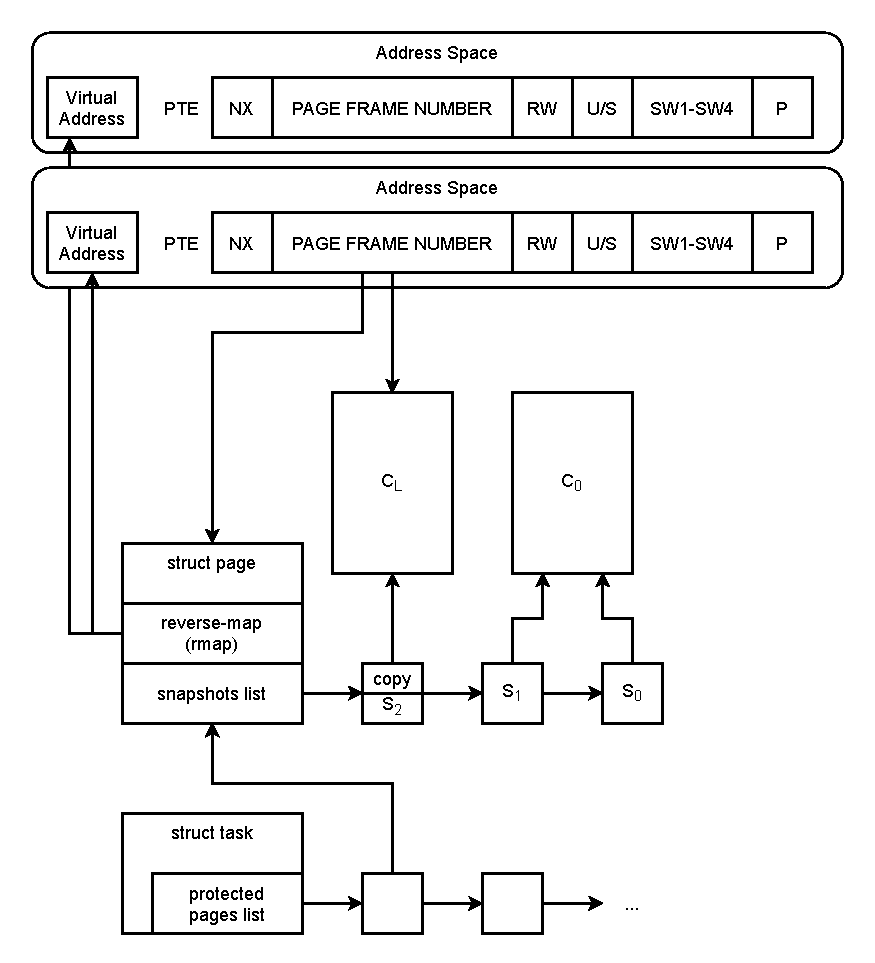
\includegraphics[width=\linewidth]{img/book-keeping.pdf}
  \caption{Bookkeeping information for a page.}
  \label{fig:tiktok_bookeeping}
\end{figure}

\tiktok needs to track the state for every userspace page, including
its snapshot and copy sets.
\autoref{fig:tiktok_bookeeping} shows the data structures used to
track this state in our prototype.
Linux maintains a \Code{struct page} object for every frame of 
physical memory. 
We augment \Code{struct page}  with a list holding the snapshots
for this page, excluding the latest snapshot $L$.
Each snapshot has a pointer to its copy. 
In the figure, the snapshots $S_1$ and $S_0$ share the copy $C_0$.
The authors are aware of the strong aversion of the 
Linux kernel developer community towards increasing the size of 
\Code{struct page}. 
An alternate implementation can use a hashmap to
map from a page's frame number to its snapshots list or
reuse existing data members (e.g., \Code{struct list_head lru} which 
can be used as a generic list by page owners).

Each pagetable entry for a user page in different address spaces 
maps the copy $C_L$, enabling userspace to directly access the page
with reads (and writes for writable pages).
We use one software-controlled bit (SW3) in the pagetable entries 
to track the protection status of the page, and another 
(SW2)\footnote{The SW2 bit is alternatively used by the experimental Software Dirty Pages feature of 
Linux, and cannot be run alongside \tiktok in our prototype.}
to track the original protections for the page. 
SW3 is set whenever the page is in one of the two protected
states (1 and 3).
On a write-triggered protection fault, SW3 can be read to 
efficiently determine if the fault was due to \tiktok's protection 
mechanisms, triggering a state change, or due to buggy software
accessing a page with illegal permissions, triggering a signal to 
the task.
Other architectures might have fewer software-usable 
bits in the page-table, and implementations of \tiktok would 
require storing the protection status of pages in a separate data structure.
The duplication status of the page is implicitly encoded in the 
snapshots: the page is duplicated when any of its snapshots
holds a pointer to a copy other than $C_L$.

Changing the protection state of pages requires PTE updates
for the page in all address spaces where the page is mapped.
The page's \Code{struct page} structure includes a reverse-map
listing for all of these pages, and the corresponding virtual
address in each.
Our prototype uses this mapping to change PTE permissions across
all address spaces for a page.


\subsection{Kernel Reads from User Memory}
%%%%%%%%%%%%%%%%%%%%%%%%%%%%%%%%%%%%%%%%%%

\begin{figure}[]
  \centering
  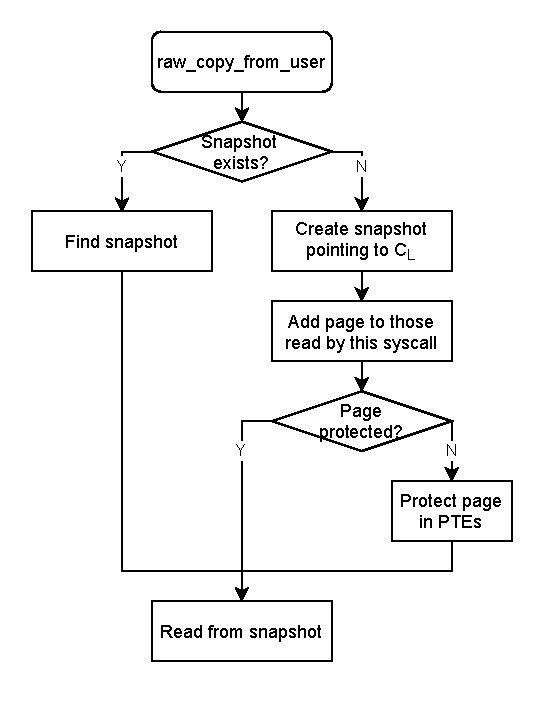
\includegraphics[width=0.8\linewidth]{img/copy_from_user.pdf}
  \caption{Flowchart for syscall reading from userspace.}
  \label{fig:copy_from_user}
\end{figure}

Syscalls reading from user memory the first time triggers the 
allocation of a new snapshot. 
If the page is not protected (states 1 and 3), the read also 
triggers a state change where the kernel protects the page
in all address space that it is mapped in. 
\autoref{fig:copy_from_user} shows the flowchart of the steps
implemented by the kernel function \Code{raw_copy_from_user} for 
reading from user memory.
This function also uses the kernel's \Code{mark_page_accessed} 
interface to move the page to the ``Active'' state for the 
kernel's swapping mechanism, making the page ineligible for being 
swapped out. 

\paragraph{Exemptions}
Our prototype \tiktok kernel exempts a couple of functions 
from \tiktok's invariant, and they are therefore not instrumented 
to follow the aforementioned steps while accessing userspace
memory. 
\Code{raw_copy_from_user_inatomic} is used by the kernel to 
read user memory in special situations such as a kernel 
oops\footnote{A kernel oops is triggered when the kernel detects a 
problem while running which can affect its proper functioning, such 
as corrupted data structures. 
A more severe version, a kernel panic, causes the kernel to stop 
executing, expecting data loss or damage if it does.}
where the kernel reads user memory to provide a backtrace. 
In this severe situation, the goal of the kernel is to collect debug 
information before its imminent termination and no \tocttou protection 
is needed.
In our prototype, we also exempt the \Code{write} system 
call's read from user memory from instrumentation.
The \Code{write} system call takes three arguments: a 
file-descriptor passed as a register, a pointer to a user 
buffer and a count of bytes to be written to the file.
While the write to the file's pages is sensitive, and 
\tiktok takes care to ensure that it follows the page state 
machine, the read from userspace is not. 
The syscall reads from userspace only once, and its data 
is only used for copying into the file.
An adversary who modifies the user buffer concurrently with 
the syscall only manages to change the contents written to 
file, which it could have done anyway since it has access to 
this buffer.
A kernel developer can similarly exempt other syscall which 
they can prove to be secure from double-fetch bugs.


\subsection{Handling Faults}
%%%%%%%%%%%%%%%%%%%%%%%%%%%%

\begin{figure}[h]
  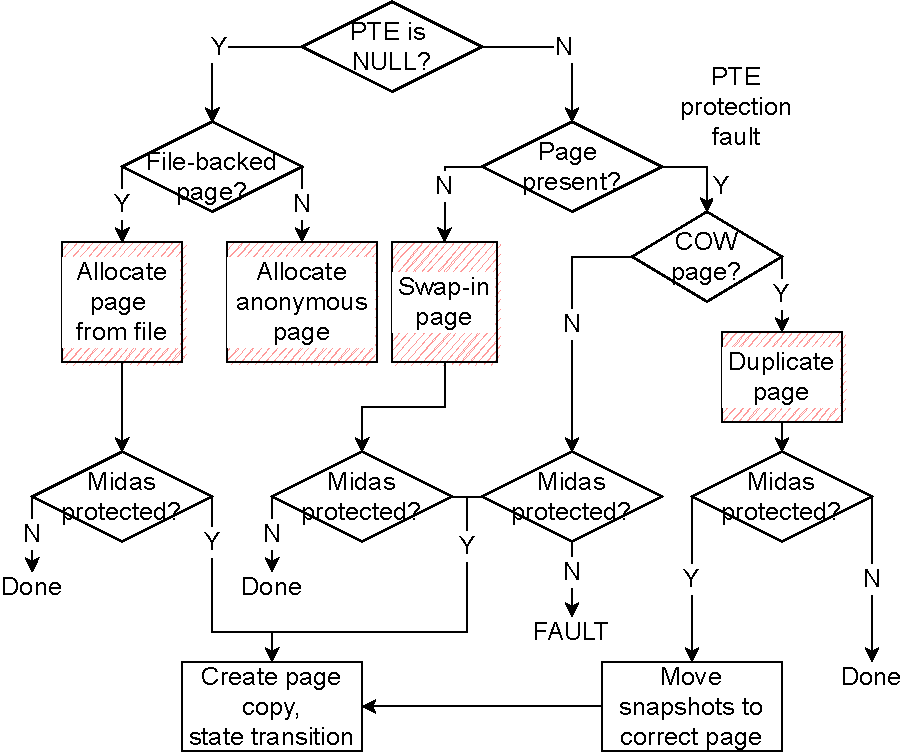
\includegraphics[width=\linewidth]{img/pagefault.pdf}
  \caption{Flowchart for handling a page fault. Shaded 
          operations are unmodified.}
  \label{fig:fault_handling}
\end{figure}

\begin{figure}[h]
  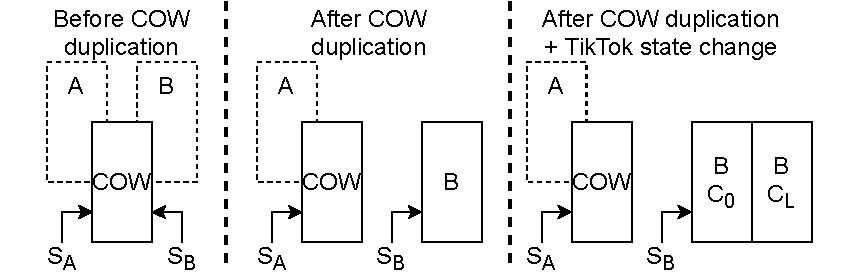
\includegraphics[width=\linewidth]{img/pagefault_cow.pdf}
  \caption{Flowchart for handling a page fault to a COW page.}
  \label{fig:fault_handling_cow}
\end{figure}

\paragraph{Handling Faults}
The memory management unit generates a fault when kernel or user code accesses
a page without having the correct permission in the corresponding PTE.
\tiktok marks writable pages read-only to protect them in 
states 1 and 3, allowing the kernel to detect writes to these pages.
A common OS mechanism, copy-on-write (COW) pages, also uses 
permissions in the PTE to detect when COW pages need to be copied.
The PTE's present bit are used to store pointers to file-backed pages
when they are swapped to disk.
\autoref{fig:fault_handling} shows the flowchart implemented by
\Code{handle_pte_fault} to handle faults for userspace addresses.

The page-fault handler first checks if the PTE is NULL, and if so 
knows that it has to allocate a page. 
If the required page is anonymous, the page can be allocated as usual.
Otherwise, for file-backed pages, the handler has to check if the 
page is already in a protected state (states 1 and 3) by reading 
the SW3 bit of the PTE and if so, transitions to the required state
and allocates a new copy. 
Pages in states 0 and 2 can be directly mapped, and subsequently
accessed.

For non-NULL PTEs, the handler checks if the PTE indicates that the 
page is present.
Non-present pages are swapped-in as usual.
Otherwise, \tiktok checks if the page was previously swapped in by 
any other task and is now in a protected state.
If not, the swap proceeds as usual.
For protected pages, \tiktok implements a state change based on 
whether the access causing the fault was a read or a write.

In the remaining case, faults for a present page indicate a 
permission fault (write to a read-only page).
If the page is not a COW-page, the handler then checks if the page
is in a protected state by checking the SW3 bit.
If the page was protected, a new copy is allocated and the page 
transitions to the following state.
For non-protected pages, however, the fault implies a real access
violation, sending a signal to the process.

COW pages represent separate virtual pages from different 
address spaces mapped to the same physical page.
An example of a COW page protected by \tiktok is illustrated in 
\autoref{fig:fault_handling_cow} where logically separate pages A and B 
are actually mapped to the COW page.
A COW page cannot be in states 2 or 3, since they cannot have multiple
\tiktok copies.
COW pages in state 0 can be dealt with by the kernel's standard
duplication method (not \tiktok's duplication).
For a COW page in state 1, its list of snapshots can correspond to 
reads from syscalls for threads in different address spaces.
In \autoref{fig:fault_handling_cow}, we show snapshots $S_A$ and 
$S_B$ corresponding to syscalls for threads in different address 
spaces (containing A and B respectively).
These snapshots correspond to different logical pages, but are 
all squashed into the snapshots list of the single COW page. 
Therefore, after the kernel duplicates the COW page (new page
B created, in \autoref{fig:fault_handling_cow}), \tiktok moves 
the snapshots for the faulting process ($S_B$) to the new page.
Here, \tiktok also updates the protected page list in the 
affected syscalls' \Code{task_struct}s so that they point to the 
new page.
Finally, the new page is transitioned to its next state to allow 
for the write to occur, creating a new copy ($C_0$) for the
snapshot $S_B$ to read from.


\subsection{Syscall Completion}
%%%%%%%%%%%%%%%%%%%%%%%%%%%%%%%

On syscall completion, \tiktok cleans up snapshots allocated for 
the syscall by instrumenting the end of \Code{do_syscall_64}.
\tiktok goes through the list of all the pages for which the 
executing syscall has a snapshot, and frees those snapshots.
For snapshots which were the last to point to a copy, that 
copy is also freed.


\subsection{File System Writes}
%%%%%%%%%%%%%%%%%%%%%%%%%%%%%%%

\tiktok instruments file-system writes to protect the kernel
from modifications via kernel mappings.
When a \Code{write} syscall writes to a file, it actually
writes to copies of pages of the file stored in memory within 
a page cache.
In the spirit of abstraction, the kernel does not directly write to 
these pages, but calls the relevant file-system (FS) driver instead.
When writing to pages in the page cache, the FS driver will access the 
page using kernel mappings.
Since \tiktok only protects userspace mappings for protected pages, 
writes by FS drivers will not raise a fault.
To comprehensively protect the page, any implementation needs to 
instrument FS-drivers' write functions.
Fortunately, FS drivers provided with the kernel follow a simple 
recipe: for pages not in the page cache, the driver executes 
FS-specific code to read the page into the page cache and then 
call a generic function (\Code{generic_file_write_iter}) to actually 
write the data into the page.
Instrumenting this generic function, therefore, protects the kernel
for a wide range of common file-systems (including ext4, nfs and 
ntfs). \footnote{A more comprehensive list of kernel-provided FS drivers 
protected via \Code{generic_file_write_iter} includes v9fs, ADFS, AFFS, 
AFS, BFS, CIFS, eCryptfs, extFAT, ext2, F2FS,  FAT, FUSE, HFS, HFS+, 
hostfs, HPFS, JFS, JFFS2, Minix, NILFS2, OMFS, OrangeFS, ramfs, ReiserFS,
SystemV, UBIFS, UDF, UFS, VboxSF, shmem.}
The added instrumentation checks whether the target page is 
protected, and if so, transitions it to the next state and 
creates a copy of the page before writing to the latest copy.

Our current prototype does not, however, protect out-of-tree drivers
which are not distributed with the kernel if they do not use the 
\Code{generic_file_write_iter} function.
A user with superuser privileges can load a module implementing a 
different, insecure FS driver which does not implement \tiktok checks.
A malicious superuser is, however, outside our threat model.
% Mat: IMO a very weak argument and always the case, so rather than waste
% precious time here, I've commented out the below as it distracts from our key
% argument IMO.
%
% A more reasonable threat involves a sysadmin unwittingly loading a 
% insecure driver which a non-privileged user can then use to 
% exploit a \tocttou bug. 
% One solution would be for the kernel to inspect the relocations table of 
% a new module while loading it to see if it uses \Code{generic_file_write_iter}
% and raising a warning if it does not.


\subsection{New Mappings to Protected Pages}
%%%%%%%%%%%%%%%%%%%%%%%%%%%%%%%%%%%%%%%%%%%%

Our \tiktok prototype preserves the state machine for user pages
across operations which create new mappings to a page to prevent 
attacks which rely on mappings being created between double fetches.
The \Code{mmap} syscall is responsible for creating new virtual
memory mappings for processes, and requires instrumentation.
When \Code{mmap} is called with the \Code{MAP_POPULATE} flag, or 
on the first access to the page, the \Code{mm_populate} function 
is responsible for actually mapping the correct page in the 
page table. 
In our prototype, we check if the page being mapped is protected, 
and if so, correctly protect the new mapping too.
Another syscall, \Code{clone}, duplicates a process' address space
when called without the \Code{CLONE_VM} flag creating new mappings
to mapped pages. 
We instrument \Code{clone} to ensure that new mappings for protected 
pages are also correctly protected.


\subsection{Discussion}
%%%%%%%%%%%%%%%%%%%%%%%

\paragraph{Optimizations on capable hardware}
To protect a page in an address space, a \tiktok implementation 
needs to change the permissions in the page table for that page.
Modern CPUs cache virtual memory translations in per-core 
Translation Lookaside Buffers (TLBs) which need to be (partially) 
flushed on page-table updates (TLB shootdown).
On most CPUs, the core updating permissions will perform a global 
shootdown to ensure that other TLBs for cores executing in the 
same address space are also updated.
Implemented with inter-processor interrupts, global shootdowns 
are expensive and account for the majority of \tiktok overhead.

A more efficient solution would be to have special hardware support
for invalidating TLB entries globally, not just on the executing 
core. 
The AMD64 architecture manual~\cite{amd64prog} lists such an instruction 
(\Code{INVLPGB}), though it is yet to be implemented in any commercially 
available x86 processors.
The ARM v8-A architecture manual~\cite{armv8a} lists similar instructions 
\Code{TLBI ASIDE1IS} and \Code{TLBI ASIDE1OS} which invalidates all entries 
of a page within a cluster of cores but not for cores in other clusters
(called an Inner Shareable Domain) and cores across clusters (called an 
Outer Shareable Domain) respectively.
Alternate architectures with a single, system-wide translation 
table~\cite{guptarebooting,ChaseLFL94} 
would also benefit \tiktok by having a single page table to 
update instead of multiple page tables for each address space a page
is mapped in.


%%%%%%%%%%%%%%%%%%%%
\section{Evaluation}
%%%%%%%%%%%%%%%%%%%%

In this section, we quantify \tiktok's overhead on workloads 
with different characteristics, both compute-bound applications
which rarely use syscalls and I/O-bound applications which 
heavily rely on the kernel's I/O interface.
\tiktok's overhead depends on the number of address spaces 
where protected pages are mapped. 
Relevant benchmarks where we expect overhead therefore include multiprocessing,
parallel benchmarks.

We evaluate \tiktok on two benchmark suites: the NAS Parallel 
Benchmark (NPB)~\cite{npb} and select workloads from the 
Phoronix Test Suite (PTS)~\cite{pts}. 
NPB includes CPU-bound multiprocessing workloads with a 
low, but non-negligible syscall rate. 
NPB therefore demonstrates the ability of \tiktok to 
scale to systems where pages are protected across numerous 
address spaces.
PTS includes a variety of benchmarks, both CPU-bound and 
I/O bound representative of both desktop and server workloads.
PTS includes syscall-heavy applications with varying degrees 
of parallelism.
We do not include the SPEC CPU2017 benchmarks
as they are heavily CPU bound and designed to isolate userspace 
performance without syscalls, and therefore do not test kernel 
performance. SPEC CPU2017 benchmarks would unfairly bias performance in favor of
\tiktok.

The testbench for the evaluation consists of a desktop machine 
with an 8-core Intel i7-9700 processor and 16GB DRAM running 
Ubuntu 20.04 LTS. This configuration and CPU is commonly used on desktop
machines and workstations.
%
To eliminate the effect of dynamic frequency and voltage 
scaling (DVFS), we set the processor to run at constant 
frequency of 3.0GHz which is this model's base frequency.
In the \emph{baseline} configuration, we run the testbench 
with the mainline kernel v5.11 available from Ubuntu's package 
repository.
The \emph{\tiktok} configuration runs our prototype \tiktok kernel 
based on kernel v5.11.
For particular benchmarks, we also run the \emph{\tiktok{+}write}
configuration which also runs our prototype \tiktok kernel
but instruments all syscalls including \Code{write}.


\subsection{NAS Parallel Benchmarks}
%%%%%%%%%%%%%%%%%%%%%%%%%%%%%%%%%%%%

\begin{figure}[]
  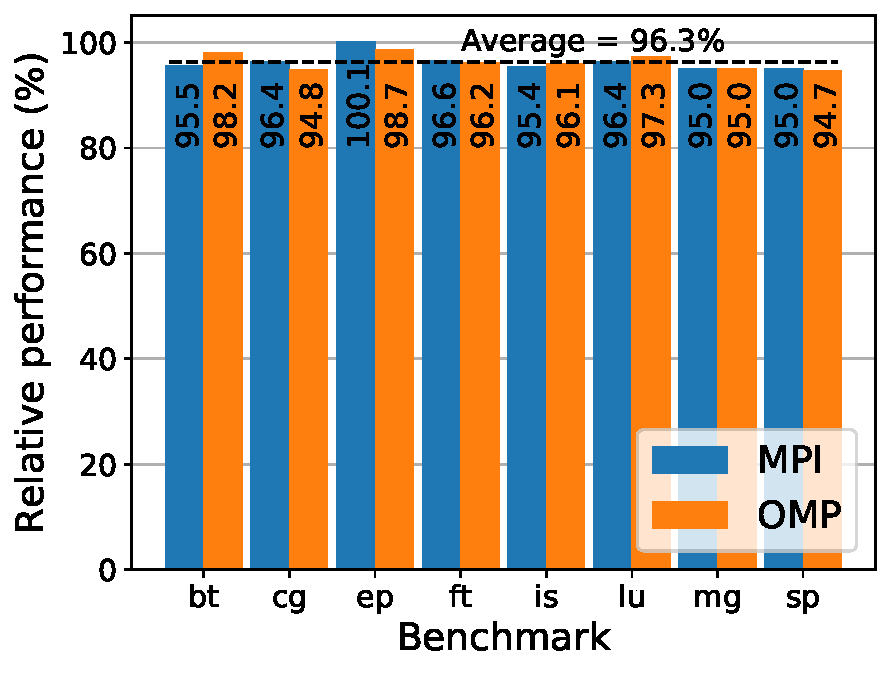
\includegraphics[width=\linewidth]{img/npb_performance.pdf}
  \caption{\tiktok performance on NPB benchmarks relative to the baseline 
          system with the same parallelization framework.}
  \label{fig:npb_performance}
\end{figure}

NAS Parallel Benchmarks (NPB)~\cite{npb} is a benchmark introduced by
NASA. 
NPB consists of several parallel programs using different communication
patterns and is available for two frameworks for parallel programming:
OpenMP and MPI.
% Two variants that test either threads or processes
OpenMP~\cite{dagum1998openmp} is a compiler extension that splits a 
program's execution to multiple threads. 
All threads still use the same address space, keeping the overhead minimal. 
MPI~\cite{snir1998mpi} implements parallel execution by launching multiple
processes which communicate by message-passing. 
The two technology stacks have different frequency of syscalls due to 
different communication methods.
Communication through kernel syscalls for either stack will incur overhead
due to \tiktok's protection.
Additional global TLB shootdowns (for snapshot synchronization) added by 
\tiktok will also affect the performance of such parallel benchmarks.

We evaluated NPB benchmarks of class A on our testbench, running 
4 threads/processes in parallel.
These benchmarks' runtime varies between 10 seconds and 8 minutes, 
and are all long enough for the kernel to reach equilibrium.
Certain benchmarks require a parallelism number which is a perfect square.
On our 8-core CPU, having 4 CPU-bound threads/processes instead of 16 allows 
all of them to run without time-sharing.
\autoref{fig:npb_performance} shows \tiktok's performance for both MPI and OpenMP,
normalized to the performance of the baseline system with the same parallelization
framework.
On average, \tiktok achieved $96.3\%$ of the baseline system's performance on 
both frameworks. 
\tiktok's performance for the \Code{ep} (Embarrassingly Parallel) benchmark is 
closest to that of the baseline, since it has low communication overheads.
\tiktok shows negligible overhead ($3.7\%$) for CPU-bound workloads, even when they 
involve parallelism.


\subsection{Phoronix Test Suite}
%%%%%%%%%%%%%%%%%%%%%%%%%%%%%%%%

\begin{figure}[]
  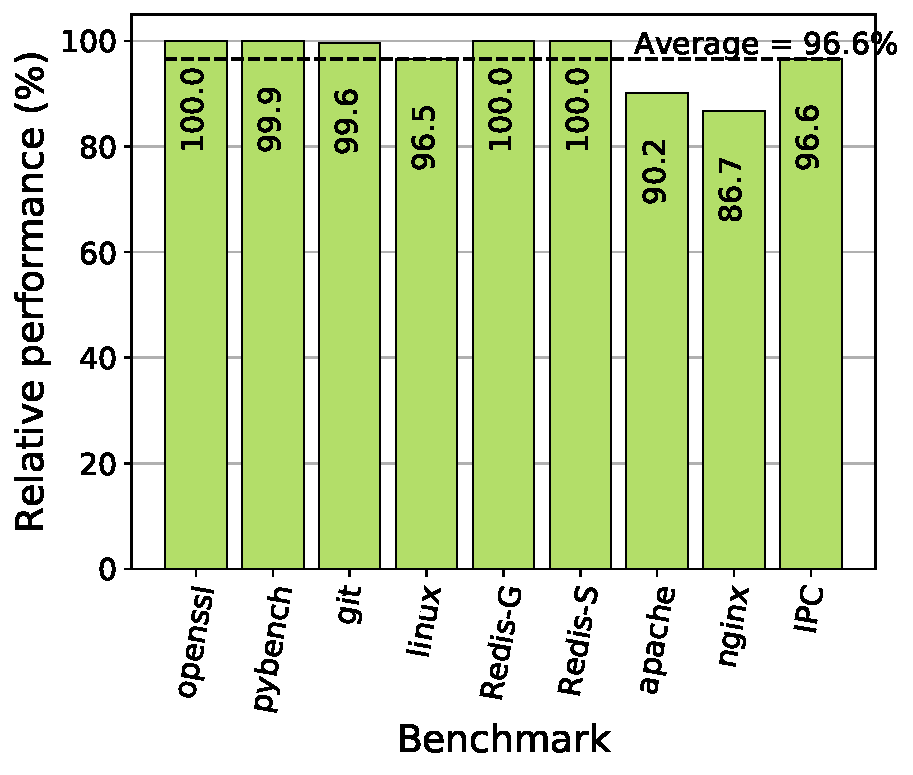
\includegraphics[width=\linewidth]{img/pts_performance.pdf}
  \caption{\tiktok performance on PTS benchmarks relative to the baseline system.}
  \label{fig:pts_performance}
\end{figure}

The Phoronix Test Suite (PTS)~\cite{pts} includes a large set ($>500$) of 
open-source benchmarks, of which we have chosen a range of benchmarks 
suitable for evaluating both desktop and server performance.
We biased the selection to benchmarks that require (heavy) kernel activity to
test the overhead of \tiktok's instrumentation.
A sole benchmark, OpenSSL, is chosen to represent single-threaded, 
CPU-bound workloads for which kernel performance is less relevant.
The benchmarks are also varied, ranging from single-threaded (Pybench) to 
multi-threaded, multi-process workloads (Apache).
At the extreme, we have an IPC benchmark transferring tiny, 128-byte 
buffers between processes which spends all of its time in syscalls
and whose performance is entirely dependent on kernel IPC performance.

We plot \tiktok's performance relative to the baseline kernel on
these benchmarks in \autoref{fig:pts_performance}, roughly ordered 
workloads in increasing order of syscall dependence from left to right.
For benchmarks for which PTS reports runtime, we compute the inverse 
of the runtime as performance.
Benchmarks with low syscall frequency such as OpenSSL, 
Pybench and Git have correspondingly low dependence on kernel performance.
Accordingly, these benchmarks see a negligible overhead when running 
on our prototype kernel.
The benchmark titled ``Linux'' represents compilation of the Linux kernel.
While compilation is mostly CPU bound, compiling the Linux kernel requires 
accessing a large number of source files, resulting in the creation 
of a large number of compiler processes each of which read and create 
different files. 
\tiktok experiences a small, but non-negligible overhead of $4\%$ on this workload.
Redis requires syscalls for receiving and replying to requests, but 
processes its transaction entirely in-memory. 
While early prototypes of our kernel caused significant degradation
of Redis' throughput (up to $69\%$), demonstrating Redis' dependence 
on kernel performance, 
our evaluation prototype achieves almost identical results as the baseline, 
highlighting the prototype's competitive performance.
The webservers, Apache and Nginx require network and file-system I/O, 
and rely heavily on syscall performance. 
We see that Nginx, which is a higher-performance webserver, sees a larger
overhead.
Fs-mark, which accesses a file system with 5000 files of 1MB concurrently
from 4 threads, and IPC, which implements 128 byte transfers between 
two processes over a TCP connection, are almost entirely bound by kernel 
performance. 
These benchmarks see a performance overhead of up to $10\%$ on \tiktok.

Our prototype \tiktok kernel benefits significantly from 
exempting particular, proven-safe syscalls from instrumentation.
While we exclude \Code{write}-like syscalls from \tiktok because they 
are not vulnerable to double-fetch bugs, we also evaluated the
performance cost of an unoptimized implementation (\tiktok{+}write)
which also instruments these syscalls.
To highlight the worst-case performance of the unoptimized implementation, 
we evaluate the performance of the IPC benchmark on \tiktok{+}write due 
to its high frequency of \Code{write} syscalls.
With \tiktok{+}write, the performance of the IPC benchmark falls to 
$12.6\%$ of the baseline, a further degradation of $81\%$ compared 
to \tiktok, showing that developer effort towards properly exempting 
frequently called \emph{safe} syscalls from \tiktok protections is crucial
towards for implementations to maintain competitive performance
compared to the baseline.

Our prototype incurs memory overhead due to metadata tracking page snapshots
and page copies. 
At any instant, the memory overhead mainly depends on the number of executing 
syscalls (limited by the core count) and the number of page copies for these 
syscalls.
On average, for every 1000 syscalls issued by the PTS benchmarks, our prototype
created 236 snapshots (32B each) and 54 copies (4KB each).
We can see that the occurrence of copies is low, resulting in negligible 
memory overhead.


%%%%%%%%%%%%%%%%%%%%
\section{Conclusion}
%%%%%%%%%%%%%%%%%%%%

\tiktok mitigates double-fetch bugs in system calls and protects the operating
system kernel by enforcing a core invariant:  \emph{through a syscall's
lifetime, every read to a userspace object will return the same value}.
Our \tiktok implementation creates on-demand snapshots and copies of pages that
are read and merges any writes through the execution of the system call.
%
Our mitigation protects the core kernel, as well as drivers by carefully
instrumenting functions that interact with the process address space. While our
implementation focuses on Linux for x86-64, our concept is generic and empowers
other kernels to protect themselves against notoriously hard-to-find and
easy-to-exploit double fetch bugs.

The performance evaluation of our prototype implementation is promising.
CPU-intensive benchmarks have negligible overhead and even syscall-intensive
benchmarks exhibit low overhead. On one hand, \tiktok mitigates all double fetch
bugs in the kernel and gives developers a tool to locate such bugs. On the other
hand, \tiktok sets the foundation for efficient, stateful system call filtering
and validation. 
%
We will release the source code of our
prototype as open-source and continue our interaction with the Linux kernel
community.

\bibliographystyle{plain}
\bibliography{TikTok}

%%%%%%%%%%%%%%%%%%%%%%%%%%%%%%%%%%%%%%%%%%%%%%%%%%%%%%%%%%%%%%%%%%%%%%%%%%%%%%%%
\end{document}
%%%%%%%%%%%%%%%%%%%%%%%%%%%%%%%%%%%%%%%%%%%%%%%%%%%%%%%%%%%%%%%%%%%%%%%%%%%%%%%%

%%  LocalWords:  endnotes includegraphics fread ptr nobj noindent
%%  LocalWords:  pdflatex acks
